\section{Packing finite comparisons into global prices}
\label{price:section}

Assume throughout this section that no finite win in the sense of
\cref{def:finite-win} exists.  We construct a function on all invertible
complex matrices.  Its values measure the costs of matrix calls in an
auxiliary argument; they do not make scalar multiplications free in the
circuit model.

\begin{samepage}
\begin{theorem}[Global prices under the no-win assumption]
\label{thm:prices}
There is a function
\[
 p:\bigcup_{n\geq1}\GL_n(\C)\longrightarrow[0,\infty)
\]
which vanishes exactly on the monomial matrices and has the following
properties.  For invertible matrices of the indicated sizes,
\begin{align}
 p(LAR)&=p(A)
 &&\text{if $L,R$ are monomial of width $|A|$},
 \label{price:monomial-law}\\
 p(AB)&\leq p(A)+p(B)
 &&\text{if $|A|=|B|$},
 \label{price:product-law}\\
 p(A\otimes B)&=|B|p(A)+|A|p(B),
 \label{price:tensor-law}\\
 p(A\oplus B)&=p(A)+p(B),
 \label{price:sum-law}\\
 p(A^{-1})&=p(A^{\mathsf T})=p(A).
 \label{price:symmetry-law}
\end{align}
Moreover,
\begin{equation}
 p(U)=1,\qquad U=\begin{pmatrix}1&0\\1&1\end{pmatrix}.
 \label{price:normalization}
\end{equation}
\end{theorem}
\end{samepage}

The proof first constructs prices satisfying every finite tensor-word
comparison.  Symmetrization at the end preserves the laws displayed in the
theorem; preservation of the entire original comparison family after that
averaging will not be needed.

\subsection{The comparison inequalities}

Take any tensor target
\(C_1\otimes\cdots\otimes C_a\), with \(a\geq1\) and each \(C_j\)
invertible, and any word implementing it on exactly
\(Q=\prod_j|C_j|\) coordinates.  Include in a finite list
\(A_1,\ldots,A_m\) every distinct nonmonomial matrix occurring either as a
factor or as a call; additional nonmonomial types may also be included.
Put \(q_i=|A_i|\).  If \(n_i\) factors equal \(A_i\) and the word uses
\(g_i\) calls to \(A_i\), define
\begin{equation}
 \Delta_i=n_iQ/q_i-g_i.
 \label{price:comparison-vector}
\end{equation}
Here \(n_iQ/q_i\) is the number of calls in the usual computation along
successive tensor axes.  Monomial factors and operations have no coordinate
in this vector.  The desired comparison is
\begin{equation}
 \sum_{i=1}^m\Delta_i p(A_i)\leq0.
 \label{price:comparison}
\end{equation}
There is no bound on the widths, number of factors, or lengths of words
used to define this family of inequalities.  Each individual inequality
involves finitely many types.

\begin{lemma}[Packing comparisons]
\label{price:packing}
Let \(\Delta^{(1)},\ldots,\Delta^{(R)}\in\R^m\) be any finite family of
comparison vectors, with \(m\geq1\) and the type list containing all their
nonmonomial factors and calls.  Under the no-win assumption there are no
numbers \(\lambda_r\geq0\) such that
\[
 s_i:=\sum_{r=1}^R\lambda_r\Delta^{(r)}_i>0
 \quad\text{for every }1\leq i\leq m.
\]
\end{lemma}

\begin{proof}
Suppose such a combination exists. We will choose a block-diagonal matrix
$J$ containing many copies of every $A_i$ and many identity blocks, and
compute $J^{\otimes b}$ in fewer than the usual $b|J|^{b-1}$ calls to
$J$. Its tensor sectors give disjoint places to run copies of the
comparison programs. The strict savings in every type leave room to
spread these programs over fewer time slots while preserving each
program's order.

For a slot to be one call to $J$, however, it must contain exactly the
prescribed number of calls to each $A_i$. Random start times will first
keep all slot loads below these capacities. We then fill every vacancy
with a call belonging to an identity word on separate coordinates.
The construction must therefore provide both slack in each slot and
enough unused coordinates for these identity words. We first choose
block proportions that reserve enough identity space; the strict
comparison savings will then supply the slot slack.

\paragraph{Fixed words, species, and proportions.}
Discard terms with coefficient zero.  A comparison whose target has only
monomial factors has \(\Delta^{(r)}_i=-g_i\leq0\) for every \(i\).
Discarding these terms only increases the numbers \(s_i\), so they may
also be discarded.  At least one comparison remains.  Replace every
monomial target factor by an identity of the same width.  To obtain its
new implementing word, append the inverse of that monomial along the
appropriate tensor axis.  The appended operation on the full sector is
monomial, so all nonmonomial call counts are unchanged.  Append width-one
identity factors to make every target have the same number \(b\geq2\)
of factors.  This changes neither its width nor its comparison vector.
Keep the entire original type list, including types appearing only in
some implementing words.  A type absent from every retained target would
have only nonpositive retained differences, contrary to \(s_i>0\).

There are now finitely many block species: one species for each \(A_i\),
and one identity species \(I_d\) for every required identity dimension
\(d\), including \(d=1\).  Denote this finite dimension set by
\(\mathcal D\).  By \cref{lem:generation}, for every \(i\) there is a
fixed word on \(q_i\) coordinates implementing identity using exactly
\(h_i>0\) calls to \(A_i\) and monomials.  Fix all these words and put
\(H=\operatorname{lcm}(h_1,\ldots,h_m)\).

Choose positive integers \(a_i\), each divisible by \(H\), and positive
integers \(u_d\), \(d\in\mathcal D\).  By increasing \(u_1\), arrange
that, for
\[
 w_0=\sum_iq_i a_i+\sum_{d\in\mathcal D}d u_d,
 \qquad
 \theta=\frac{\sum_iq_i a_i}{w_0},
\]
one has
\begin{equation}
 b\theta<(1-\theta)^b.
 \label{price:identity-capacity}
\end{equation}
This is possible since \(\theta\) tends to zero as \(u_1\) increases.
For each positive integer \(v\), set
\[
 w=vw_0,\quad k_i=va_i,\quad \ell_d=vu_d,\quad
 J=\bigoplus_i A_i^{\oplus k_i}
       \ \oplus\!\bigoplus_{d\in\mathcal D}I_d^{\oplus\ell_d}.
\]
Thus \(|J|=w\).  The fixed copy ratios
\(\rho_i=k_i/w=a_i/w_0\) and \(\gamma_d=\ell_d/w=u_d/w_0\)
are all strictly positive.  We let \(w\) tend to infinity only along
these multiples of \(w_0\).  In particular every \(k_i\) is divisible
by \(H\), and the active coordinate fraction is exactly
\(\sum_iq_i\rho_i=\theta\).

The block decomposition of \(J^{\otimes b}\) has one sector for every
choice of a block copy on each of its \(b\) axes.  A sector with species
pattern \(\sigma=(\sigma_1,\ldots,\sigma_b)\) has width equal to the
product of those species' widths.  Write \(\tau_{A_i}=\rho_i\) and
\(\tau_{I_d}=\gamma_d\).  The exact number of sectors with that ordered
pattern is
\begin{equation}
 \prod_{j=1}^b (w\tau_{\sigma_j})
     =\beta_\sigma w^b,
 \qquad \beta_\sigma=\prod_{j=1}^b\tau_{\sigma_j}>0.
 \label{price:sector-count}
\end{equation}
Repeated species give ordinary powers in this product: choices on distinct
tensor axes are independent, so the same block-copy label can occur on
two different axes.  Patterns differing in any species have disjoint
sector sets.

\paragraph{Disjoint replacements and a fixed saving.}
Let \(\sigma(r)\) be comparison \(r\)'s ordered target pattern.
Choose a fixed \(\eta>0\) sufficiently small that
\begin{equation}
 \eta\sum_{r:\,\sigma(r)=\sigma}\lambda_r
       \leq \tfrac12\beta_\sigma
 \quad\text{for every used pattern }\sigma,
 \qquad
 \eta s_i\leq\tfrac12 b\rho_i\quad(1\leq i\leq m).
 \label{price:eta-choice}
\end{equation}
All quantities on the right have already been fixed and are positive.
For comparison \(r\), select
\[
 m_r(w)=H\left\lfloor\frac{\eta\lambda_r w^b}{H}\right\rfloor
\]
sectors of pattern \(\sigma(r)\).  Equation~\eqref{price:eta-choice}
ensures that all selections can be disjoint, including selections of
different comparisons having the same pattern.  Run the comparison's
word on each selected sector.  On every other sector run the standard
axis program.  Sectors containing only identity species require no
operation, and no such sector was selected.

The standard sector programs would use
\(G_i^0=b k_iw^{b-1}\) calls to \(A_i\): choose the axis, one of its
\(k_i\) copies of \(A_i\), and one coordinate on each remaining axis.
The programs after replacement use
\begin{align}
 G_i
 &=b k_iw^{b-1}-\sum_rm_r(w)\Delta^{(r)}_i \notag\\
 &=(b\rho_i-\xi_i)w^b+E_i(w),
 \qquad \xi_i=\eta s_i>0,
 \label{price:total-load}
\end{align}
where
\( |E_i(w)|\leq H\sum_r|\Delta^{(r)}_i|\).
In particular \(G_i\) is a nonnegative integer divisible by \(H\).
There are only finitely many possible standard sector patterns and
replacement words.  Hence there is a fixed integer \(L\geq1\) bounding
the number of nonmonomial calls in every such program, independently of
\(w\).  Monomials before, between, and after these calls are retained as
part of the program.

Choose a fixed \(\eps>0\) such that
\[
 0<\eps<\min(1,b/2),\qquad
 \eps\rho_i<\xi_i/4\quad(1\leq i\leq m),
\]
and set
\[
 T=\lfloor(b-\eps)w^{b-1}\rfloor,
 \qquad F=T-L+1.
\]
For all sufficiently large \(w\), \(F>0\) and
\[
 k_i-\frac{G_i}{F}
 =\frac{\xi_i-\eps\rho_i}{b-\eps}\,w+O(w^{2-b}).
\]
The constants in the error terms are independent of \(w\).  Fix a
number \(\kappa>0\) smaller than half the minimum of the positive
coefficients in this display.  Increasing the lower threshold on \(w\)
if necessary gives simultaneously
\begin{equation}
 \frac{G_i}{F}\leq k_i-\kappa w
 \quad(1\leq i\leq m).
 \label{price:load-margin}
\end{equation}
Thus the finite comparisons, their words, \(b,h_i,H\), the species
proportions (and \(\theta\)), \(\eta,\xi_i,L\), and finally
\(\eps,\kappa\) have all been fixed before \(w\) is taken large.

\paragraph{A schedule respecting all dependencies.}
Independently for each sector program having at least one nonmonomial
call, choose a start uniformly from \(\{1,\ldots,F\}\).  Put its
successive nonmonomial calls in consecutive slots starting there.
Every call lies in \(\{1,\ldots,T\}\), and its internal order is
preserved.  For a fixed type \(i\) and slot \(t\), let \(X_{i,t}\)
be the number of scheduled calls of that type.  A given sector contributes
an indicator, even if its program uses \(A_i\) repeatedly: different
positions in that program require different starts to fall at slot
\(t\), and these events are mutually exclusive.  Its contribution has
mean at most its number of \(A_i\) occurrences divided by \(F\).
Different sectors have independent starts.  Consequently \(X_{i,t}\)
is a sum of independent Bernoulli variables with
\(\mathbb E X_{i,t}\leq G_i/F\).

For completeness, write \(\rho_{\max}=\max_i\rho_i\), and choose
\(0<a\leq1\) so small that
\((e^a-1-a)\rho_{\max}\leq a\kappa/2\).  Such a choice follows,
for example, from \(e^a-1-a\leq ea^2/2\) on \([0,1]\).
Independence, \(1+x\leq e^x\), and Markov's inequality give
\begin{align*}
 \Pr(X_{i,t}>k_i)
 &\leq e^{-ak_i}\mathbb E e^{aX_{i,t}}\\
 &\leq\exp\bigl(-ak_i+(e^a-1)(k_i-\kappa w)\bigr)\\
 &\leq\exp(-a\kappa w/2).
\end{align*}
There are \(mT=O(w^{b-1})\) pairs \((i,t)\), with fixed \(m,b\).
The union bound therefore tends to zero.  For a sufficiently large
admissible \(w\), fix one schedule for which \(X_{i,t}\leq k_i\)
for every type and every slot.  Independence between different slots is
neither claimed nor needed.

\paragraph{Completing the vacancies with identities.}
For type \(i\), the number of unfilled call positions is
\[
 D_i=k_iT-G_i.
\]
It is divisible by \(H\), hence by \(h_i\).  Moreover,
\cref{price:load-margin} gives
\[
 D_i\geq k_i(L-1)+\kappa wF=\Omega(w^b).
\]
Let \(d_i=D_i/h_i\); for sufficiently large \(w\), every \(d_i>k_i\).
Allocate \(d_i\) disjoint ordered groups of \(q_i\) wires to run the
fixed \(h_i\)-call identity word for \(A_i\).  All these groups, for
all types together, fit in the union of the all-identity sectors.  Indeed
that region has exactly \(((1-\theta)w)^b\) wires, whereas
\begin{equation}
 \sum_iq_i d_i
 \leq\sum_iq_i k_iT
 =\theta wT
 <b\theta w^b
 <(1-\theta)^b w^b.
 \label{price:dummy-capacity}
\end{equation}
We used \(h_i\geq1\) and \(G_i\geq0\) in the first inequality.
A dummy group may cross the boundaries of the original identity
sectors, since the prescribed action on their entire union is identity.

List the \(D_i\) idle positions for type \(i\) in chronological order,
with any fixed order among positions in the same slot.  Assign successive
positions cyclically to its \(d_i\) dummy groups.  Each group receives
exactly \(h_i\) positions because \(D_i=d_i h_i\).  Two successive
positions assigned to the same group are \(d_i\) places apart in this
list.  A single time contains at most \(k_i<d_i\) positions, so these
two positions have strictly increasing times.  Assign the identity
word's successive calls to these times.  This argument permits arbitrary
clustering of vacancies.  We now have exactly \(k_i\) calls to every
type \(i\) in every slot, on mutually disjoint tuples.

\paragraph{The exact word, including all monomials.}
The physical support of each active-sector program is fixed.  Dummy
groups have fixed supports disjoint from each other and from those
sectors.  Write any one of these programs chronologically as
\[
 O_{p,0},\ A_{p,1},\ O_{p,1},\ldots,
 A_{p,l_p},\ O_{p,l_p},
\]
where the \(O_{p,j}\) are monomials on that program's support.  Let its
strictly increasing call times be \(t_{p,1},\ldots,t_{p,l_p}\).
Place \(O_{p,0}\) in the gap immediately before \(t_{p,1}\), and place
\(O_{p,j}\), \(j\geq1\), in the gap immediately after \(t_{p,j}\).
This is always before its next call, including when the times are
consecutive.  A program with no calls can place its single monomial in
the initial gap.  Operations in a gap on different program supports
combine into one ambient monomial \(M_t\), where gap \(t\) follows
slot \(t\), and gap zero precedes slot one.  A sector monomial may
permute all values on its support.  Subsequent calls still use the fixed
tuple indices prescribed by that same program, so this causes no change
to the program's meaning.

Let \(B_t\) be the simultaneous calls in slot \(t\).  There are
exactly \(k_i\) ordered tuples for each \(A_i\).  Match them bijectively
to the corresponding active blocks of \(J\).  Their union has
\(\sum_iq_i k_i=\theta w\) wires.  Complete this matching to an
injection of all \(w\) coordinates of \(J\) by using
\((1-\theta)w\) further distinct wires as spectators for its identity
blocks.  There are enough: the ambient width is \(w^b\geq w\).
Extend the matching to a permutation \(P_t\) of all ambient wires.
With the convention that \(P_t\) gathers into the canonical first
\(w\) positions, one has exactly
\begin{equation}
 B_t=P_t^{-1}\bigl(J\oplus I_{w^b-w}\bigr)P_t.
 \label{price:gather-scatter}
\end{equation}
The conjugate acts by the requested \(A_i\) on every called tuple and
fixes every other physical wire pointwise.  In particular a spectator
can belong to an unfinished sector program or dummy word: both its value
and its location are preserved by the complete gather--call--scatter
operation.  \Cref{price:packing-diagram} shows the chronological slots
and the gather--call--scatter realization of each $B_t$.

\begin{figure}[tb]
\centering
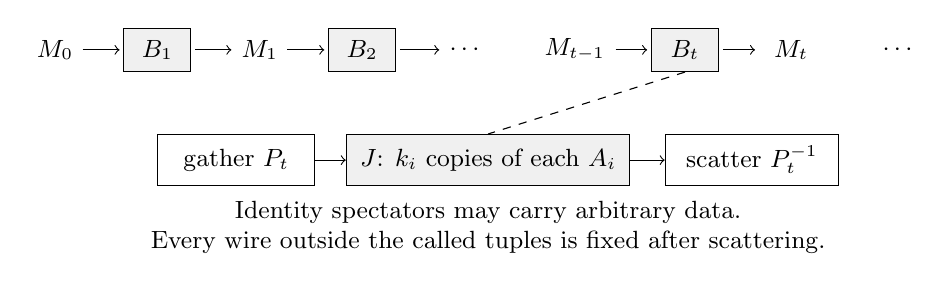
\begin{tikzpicture}[x=1cm,y=1cm, every node/.style={font=\small}]
 \node at (0,1.35) {$M_0$};
 \node[draw,fill=gray!12,minimum width=.85cm,minimum height=.55cm] (b1) at (1.3,1.35) {$B_1$};
 \node at (2.6,1.35) {$M_1$};
 \node[draw,fill=gray!12,minimum width=.85cm,minimum height=.55cm] (b2) at (3.9,1.35) {$B_2$};
 \node at (5.2,1.35) {$\cdots$};
 \node at (6.6,1.35) {$M_{t-1}$};
 \node[draw,fill=gray!12,minimum width=.85cm,minimum height=.55cm] (bt) at (8,1.35) {$B_t$};
 \node at (9.35,1.35) {$M_t$};
 \node at (10.7,1.35) {$\cdots$};
 \draw[->] (.35,1.35)--(.82,1.35);
 \draw[->] (1.78,1.35)--(2.24,1.35);
 \draw[->] (2.95,1.35)--(3.42,1.35);
 \draw[->] (4.38,1.35)--(4.88,1.35);
 \draw[->] (7.12,1.35)--(7.52,1.35);
 \draw[->] (8.48,1.35)--(8.89,1.35);
 \node[draw,minimum width=2cm,minimum height=.65cm] (g) at (2.3,-.05) {gather $P_t$};
 \node[draw,fill=gray!12,minimum width=3.6cm,minimum height=.65cm] (j) at (5.5,-.05) {$J$: $k_i$ copies of each $A_i$};
 \node[draw,minimum width=2.2cm,minimum height=.65cm] (s) at (8.85,-.05) {scatter $P_t^{-1}$};
 \draw[->] (g.east)--(j.west);
 \draw[->] (j.east)--(s.west);
 \draw[dashed] (bt.south)--(j.north);
 \node[align=center] at (5.5,-.9) {Identity spectators may carry arbitrary data.\\
 Every wire outside the called tuples is fixed after scattering.};
\end{tikzpicture}
\caption{Chronological gaps preserve each local word.  Each simultaneous
call slot is one embedded $J$ call with its gather and scatter permutations.}
\label{price:packing-diagram}
\end{figure}

Thus the matrix product
\begin{equation}
 M_TB_TM_{T-1}\cdots M_1B_1M_0
 \label{price:assembled-word}
\end{equation}
restricts to the prescribed program on every active sector and to
identity on every dummy group and unused identity wire.  It is exactly
\(J^{\otimes b}\).  By \cref{price:gather-scatter} it uses precisely
\(T<bw^{b-1}\) calls to \(J\), with all remaining operations monomial,
on precisely \(w^b\) wires.  Since at least one \(A_i\) occurs in
\(J\), the matrix \(J\) is nonmonomial.  This is a finite win,
contrary to the assumption.
\end{proof}

\subsection{Separation, normalization, and compactness}

For a nonempty finite comparison family on a nonempty finite type list,
\cref{price:packing} says that the convex hull of its difference vectors
is disjoint from the open positive orthant \((0,\infty)^m\).
Finite-dimensional separation supplies a nonzero vector \(v\) and a
real number \(c\) with
\[
 v\cdot\Delta^{(r)}\leq c\leq v\cdot y
 \quad\text{for all $r$ and all }y\in(0,\infty)^m;
\]
see \citet[Section~2.5.1, p.~46]{boydVandenberghe2004}.
If a coordinate of \(v\) were negative, sending that coordinate of
\(y\) to infinity would contradict the lower bound by \(c\).
Thus \(v\geq0\).  The infimum of \(v\cdot y\) on the positive
orthant is zero, so \(c\leq0\).  We have obtained nonnegative prices,
not all zero, satisfying every comparison in the finite family.
For an empty family any nonzero nonnegative vector suffices.

We next prevent the normalization from escaping along different types.
Include the fixed shear \(U\) of \cref{price:normalization} in every
finite type list.  For each nonmonomial \(A\) of width \(q\), fix the
following two words once and for all.  Gaussian elimination implements
\(A\) by a finite positive number \(C_A\) of embedded \(U\)-calls
and monomials.  Indeed row permutations and nonzero row scalings are
monomial, and every nonzero row addition is a diagonal conjugate of an
ordered \(U\)-call.  The comparison with one-factor target \(A\)
imposes
\[
 p(A)\leq C_Ap(U).
\]
On width \(2q\), apply \cref{lem:generation} to
\(A\oplus I_q\).  Its calls are embedded calls to \(A\), and it
generates \(U\otimes I_q\) by some fixed word with \(e_A>0\)
such calls and monomials.  The two-factor target \(U\otimes I_q\)
has standard count \(q\) for \(U\), giving
\[
 q p(U)\leq e_Ap(A).
\]
Consequently these two comparisons impose the fixed bounds
\begin{equation}
 c_Ap(U)\leq p(A)\leq C_Ap(U),\qquad c_A=q/e_A>0.
 \label{price:fixed-bounds}
\end{equation}
They introduce no new nonmonomial type other than \(A\) and \(U\).
For \(A=U\), take simply \(c_U=C_U=1\).

Augment any finite comparison family by these bounds for all its types.
Separation gives a nonzero nonnegative solution.  If its \(U\)-price
were zero, every other coordinate would be zero by the upper bounds,
which is impossible.  Divide by its positive \(U\)-price to obtain
\(p(U)=1\).  Applying this argument just to the bounds for one type
also proves that each fixed interval \([c_A,C_A]\) is nonempty.

The collection of all finite complex matrices is a set, as it is
contained in \(\bigcup_{n\geq1}\C^{n^2}\).  Form the product over
all nonmonomial invertible matrices
\[
 \mathcal P=\prod_A[c_A,C_A].
\]
Each factor is a nonempty compact interval, so this product is compact
in the product topology by Tychonov's Theorem
\citep[Tag~08ZU, Theorem~5.14.4]{stacksProject}.
Each comparison specifies a closed subset of \(\mathcal P\), since
it is a linear inequality in finitely many coordinate projections.
Any finite collection of these closed subsets has nonempty intersection:
apply the preceding finite argument to its types, include \(U\), and
augment with their fixed bounds; all other coordinates can be assigned
their lower endpoints.  Compactness gives a point satisfying every
comparison simultaneously.  Call this preliminary function \(p_0\),
and set \(p_0(A)=0\) on monomial matrices.  It is strictly positive
on each nonmonomial matrix, and \(p_0(U)=1\).

\subsection{Algebraic laws and symmetry}

We derive the laws from the comparisons before symmetrizing.  A
one-factor target \(AB\), implemented by consecutive calls to \(B\)
and \(A\), gives
\(p_0(AB)\leq p_0(A)+p_0(B)\).  This remains true if any of the
matrices is monomial, since its call is then a monomial operation of
price zero.  Multiplication by monomials on either side cannot increase
price.  Applying the same observation with their inverses shows
\(p_0(LAR)=p_0(A)\).

The standard axis program for the one-factor target \(A\otimes B\)
gives
\[
 p_0(A\otimes B)\leq |B|p_0(A)+|A|p_0(B).
\]
For the reverse inequality, use the two-factor target \(A\otimes B\)
and the word consisting of one call to that entire matrix.  Its
comparison gives the opposite inequality.  Hence the tensor law is
exact, including when a factor is an identity or any other monomial.

For direct sums the one-factor target \(A\oplus B\), implemented
by disjoint calls to its two blocks, gives
\(p_0(A\oplus B)\leq p_0(A)+p_0(B)\).  The reverse inequality
requires a separate construction.  Put \(a=|A|\), \(e=|B|\), and
\[
 X=A^{\otimes a}\otimes B^{\otimes e},\qquad Q=|X|.
\]
Consider the tensor target \(X\otimes I_2\), with its factors listed
as \(a\) copies of \(A\), \(e\) copies of \(B\), and \(I_2\).
After a coordinate permutation this is two independent copies of \(X\); this statement
is an identity of matrices and does not use a direct-sum price law.
In the first copy run all \(A\)-axes and then all \(B\)-axes.
In the second copy run all \(B\)-axes and then all \(A\)-axes.
There are exactly \(aQ/a=Q\) individual \(A\)-calls and
\(eQ/e=Q\) individual \(B\)-calls in each copy.
Pair the successive \(Q\) first-stage \(A\)-calls of the first
copy with the successive \(Q\) first-stage \(B\)-calls of the
second copy.  Each pair acts on disjoint tuples and is one embedded
\(A\oplus B\)-call, after gathering its coordinates.  Pair the
second stages in the same manner, reversing which copy supplies which
type.  Each copy retains its own required call order.  We obtain a word
with \(2Q\) calls to \(A\oplus B\), with only permutations added.
The comparison for the displayed tensor target therefore gives
\[
 2Q\bigl(p_0(A)+p_0(B)\bigr)
       \leq2Qp_0(A\oplus B).
\]
The construction also applies when one or both factors are monomial:
we may keep their individual block operations in the pairing, while
their contribution to the comparison is zero.  Thus direct-sum
additivity is established without using it to produce the two copies.

Finally define
\begin{equation}
 p(A)=\tfrac14\bigl(p_0(A)+p_0(A^{-1})
                 +p_0(A^{\mathsf T})+p_0(A^{-\mathsf T})\bigr).
 \label{price:averaging}
\end{equation}
Inversion and transposition commute and each has order two, so this
function has both symmetries.  Each of the four summands retains product
subadditivity: transposition or inversion may reverse the order of
\(AB\), but the scalar upper bound is still \(p_0(A)+p_0(B)\)
with the corresponding transforms.  They retain both exact laws because
inverse and transpose act componentwise on tensor products and direct
sums.  They retain monomial invariance, and are positive exactly on
nonmonomials, because these operations preserve the class of monomial
matrices.  Also \(U^{-1}\) is conjugate to \(U\) by
\(\diag(1,-1)\), and \(U^{\mathsf T}\) is conjugate to \(U\)
by the two-coordinate swap.  Thus every summand in
\cref{price:averaging} has value one at \(U\).  This proves
\cref{thm:prices}.  All subsequent arguments use this symmetric \(p\)
and its proved laws, without imposing additional comparison constraints
on the average.

\begin{corollary}[Shears, pairs, and embedded words]
\label{price:word-bounds}
Every nontrivial elementary coordinate shear has price one, including
with any number of untouched coordinates.  Every invertible
\(2\times2\) matrix has price at most two.  If a word on \(w\)
coordinates implements \(G\), using nonmonomial calls
\(A_1,\ldots,A_l\) and monomials, then
\[
 p(G)\leq\sum_{j=1}^l p(A_j).
\]
If the word instead implements \(G\oplus I_s\), the same bound holds
for \(p(G)\), with no restriction on the initial values of the
\(s\) coordinates restored by the word.
\end{corollary}

\begin{proof}
A shear adding a nonzero multiple of one coordinate into another is a
monomial conjugate of \(U\oplus I\), so its price is one by
\cref{price:monomial-law,price:sum-law,price:normalization}.
For an invertible pair matrix, first permute rows if needed to make its
upper-left entry nonzero.  With entries \(\alpha,\beta,\gamma,\delta\)
and determinant \(D\ne0\), it factors as
\[
 \begin{pmatrix}\alpha&\beta\\\gamma&\delta\end{pmatrix}
 =\begin{pmatrix}1&0\\\gamma/\alpha&1\end{pmatrix}
  \begin{pmatrix}\alpha&0\\0&D/\alpha\end{pmatrix}
  \begin{pmatrix}1&\beta/\alpha\\0&1\end{pmatrix}.
\]
This uses at most two nontrivial shears and a monomial.  Finally an
embedded call to \(A\) is a permutation conjugate of
\(A\oplus I_{w-|A|}\), omitting the identity block when it has size
zero, whose price is \(p(A)\).  Repeated product
subadditivity gives the word bound.  Identity padding has price zero
by direct-sum additivity.  The last assertion is an exact matrix
identity on all input coordinates; it does not assume zero scratch
values.
\end{proof}
